\documentclass[10pt,danish,t,10pt]{beamer}
\usepackage{lmodern}
\usepackage[T1]{fontenc}
\usepackage[utf8]{inputenc}
\setlength{\parskip}{\smallskipamount}
\setlength{\parindent}{0pt}
\usepackage{babel}
\usepackage{amsmath}
\usepackage{amssymb}
\usepackage{graphicx}

\usepackage{comment} % For longer notes
\ifx\hypersetup\undefined
  \AtBeginDocument{%
    \hypersetup{unicode=true}
  }
\else
  \hypersetup{unicode=true}
\fi
%\usepackage{breakurl}

\usepackage{tikzsymbols}% Smileys and stuf

\makeatletter
%%%%%%%%%%%%%%%%%%%%%%%%%%%%%% Textclass specific LaTeX commands.
% this default might be overridden by plain title style
\newcommand\makebeamertitle{\frame{\maketitle}}%
% (ERT) argument for the TOC

\AtBeginDocument{%
  \let\origtableofcontents=\tableofcontents
  \def\tableofcontents{\@ifnextchar[{\origtableofcontents}{\gobbletableofcontents}}
  \def\gobbletableofcontents#1{\origtableofcontents}
}

\usepackage{hyperref} %For link- references


\newcommand{\code}[1]{\textit{#1}} %Format for python, in case I wise for something different change textit


%%%%%%%%%%%%%%%%%%%%%%%%%%%%%% User specified LaTeX commands.
\usepackage{tikz}
\usetikzlibrary{positioning}
    
\usepackage{pgfplots}
\pgfplotsset{compat=1.17} % This sets the version, to avoid problems due to lack of backward compatibility 
\usepackage{appendixnumberbeamer}

\usetheme[progressbar=frametitle,block=fill]{metropolis}

% code
\usepackage{listings} 

% margin
\setbeamersize{text margin right=1.5cm}

% colors
\colorlet{DarkRed}{red!70!black}
\setbeamercolor{normal text}{fg=black}
\setbeamercolor{alerted text}{fg=DarkRed}
\setbeamercolor{progress bar}{fg=DarkRed}
\setbeamercolor{button}{bg=DarkRed}


% width of seperators
\makeatletter
\setlength{\metropolis@titleseparator@linewidth}{1pt}
\setlength{\metropolis@progressonsectionpage@linewidth}{1pt}
\setlength{\metropolis@progressinheadfoot@linewidth}{1pt}
\makeatother

% new alert block
\newlength\origleftmargini
\setlength\origleftmargini\leftmargini
\setbeamertemplate{itemize/enumerate body begin}{\setlength{\leftmargini}{4mm}}
\let\oldalertblock\alertblock
\let\oldendalertblock\endalertblock
\def\alertblock{\begingroup \setbeamertemplate{itemize/enumerate body begin}{\setlength{\leftmargini}{\origleftmargini}} \oldalertblock}
\def\endalertblock{\oldendalertblock \endgroup}
\setbeamertemplate{mini frame}{}
\setbeamertemplate{mini frame in current section}{}
\setbeamertemplate{mini frame in current subsection}{}
\setbeamercolor{section in head/foot}{fg=normal text.bg, bg=structure.fg}
\setbeamercolor{subsection in head/foot}{fg=normal text.bg, bg=structure.fg}

% footer
\makeatletter
\setbeamertemplate{footline}{%
    \begin{beamercolorbox}[colsep=1.5pt]{upper separation line head}
    \end{beamercolorbox}
    \begin{beamercolorbox}{section in head/foot}
      \vskip1pt\insertsectionnavigationhorizontal{\paperwidth}{}{\hskip0pt plus1filll \insertframenumber{} / \inserttotalframenumber \hskip2pt}\vskip3pt% 
    \end{beamercolorbox}%
    \begin{beamercolorbox}[colsep=1.5pt]{lower separation line head}
    \end{beamercolorbox}
}
\makeatother

% toc
\setbeamertemplate{section in toc}{\hspace*{1em}\inserttocsectionnumber.~\inserttocsection\par}
\setbeamertemplate{subsection in toc}{\hspace*{2em}\inserttocsectionnumber.\inserttocsubsectionnumber.~\inserttocsubsection\par}

\makeatother
\title{Ninth exercise class \vspace{-2mm}}
\subtitle{Class 5 \\Introduction to numerical programming and analysis \vspace{-4mm} } 
\author{Asker Nygaard Christensen}
\date{Spring 2021}

\begin{document}


{
\setbeamertemplate{footline}{} 
\begin{frame}

\maketitle

\begin{tikzpicture}[overlay, remember picture]
\node[below left=0cm and 0cm of current page.north east] 
{
\includegraphics[width=3 cm]{ku_logo.png}};
\end{tikzpicture}

\end{frame}
}

\addtocounter{framenumber}{-1}

\begin{frame}<beamer>
\frametitle{Plan}

\tableofcontents[]
\end{frame}


\section{Problem Set 5, P.2-P.4}
\begin{frame}{PS 5}
I don't have to many direct notes for problem set 5, P.2-P.4, since there are many references already.
I have uploaded my version of the answers if you're interested in \href{https://github.com/AskerNC/exercises-2021}{\underline{alternative solutions}}. There is also an faster implementation of the sieve of Eratosthenes in the last problem (which you'll need if you have a crack at project Euler). 
\end{frame}
\begin{frame}{P.2-P.4}

\begin{itemize}
    \item[P.2] \textbf{Factorical}. If recursion is messing with your mind you can watch \href{https://www.youtube.com/watch?v=Mv9NEXX1VHc}{\underline{this video}}, which is explains it quit nicely, using the factorial as an example. \\
    They also made \href{https://www.youtube.com/watch?v=8lhxIOAfDss}{\underline{this video}}, with a slightly more complicated example. 
    \item[P.3] \textbf{Bubble sort}. As noted, you can use the \code{bubble\_sort()} from the lectures, the change you have to make, is to make the function sort in descending order instead of ascending.
    \item[P.4] \textbf{Linear search}. As noted, take inspiration from \code{linear\_search()} from the lectures. And notice that this time you are not looking for an exact match
\end{itemize}
\end{frame}


\section{P.5 and P.6, intuition}
\begin{frame}{P.5-P.6}
    For \textbf{Bisection} and \textbf{Finding prime numbers} there is no corresponding functions in the lectures. So these are a bit harder. There are, however, algorithmic 'cooking recipes' to use a guide. \\
    I'll try to explain the intuition now, and then we'll go through the answer at the end of class.
    \begin{tikzpicture}[overlay, remember picture]
        \node[below left=4.5 cm and 0 cm of current page.north east] 
        {
\includegraphics[width=7 cm]{no_training_wheels.jpg}};
    \end{tikzpicture}
\end{frame}

\begin{frame}{P.5, intuition}
\begin{tikzpicture}
\begin{axis}[
title={$ f\left(x\right)=\left(2.1 \cdot   x-1.7\right)\cdot\left(x-3.3\right) \frac{1}{x^2}$},
ylabel={$f\left(x\right)$},
xtick={0,0.1,0.2,...,0.9,1},
domain=0:1,
width=10cm,
height=7cm,
]
\addplot [
    blue,
    domain=0:1,
    ] {(2.1*x-1.7)*(x-3.3)};
\addplot [
    black,
    domain=0:1,
    ] {(0)};
\end{axis}
\end{tikzpicture}
\end{frame}


\begin{frame}{P.6, intuition}
Definition of prime: A prime number is a
natural number, greater than 1 that is not a product of two smaller natural numbers.
    \begin{tikzpicture}[overlay, remember picture]
        \node[below left=3.1 cm and 0.2 cm of current page.north east] 
        {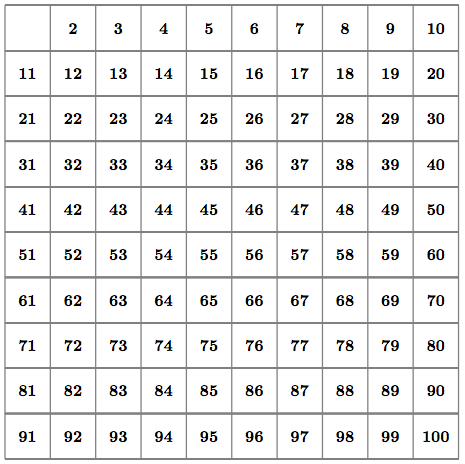
\includegraphics[width=12 cm]{sieve.png}};
    \end{tikzpicture}
\end{frame}
\section{Self work 15:40-16:45}
\section{Going through P.5 and P.6 together}

\section{Recap}
\begin{frame}{Euler}
    You're very welcome to ask my questions about Euler problems also.
    \textbf{ALSO:} Remember to do your peer feedback, they're a requirement for the exam!
    \begin{tikzpicture}[overlay, remember picture]
        \node[below left=2.35cm and 2.2 cm of current page.north east] 
        {
\includegraphics[width=7.4 cm]{limited_by_my_time.jpg}};
    \end{tikzpicture}
\end{frame}


\end{document}